\let\negmedspace\undefined
\let\negthickspace\undefined
\documentclass[journal]{IEEEtran}
\usepackage[a5paper, margin=10mm, onecolumn]{geometry}
%\usepackage{lmodern} % Ensure lmodern is loaded for pdflatex
\usepackage{tfrupee} % Include tfrupee package

\setlength{\headheight}{1cm} % Set the height of the header box
\setlength{\headsep}{0mm}     % Set the distance between the header box and the top of the text

\usepackage{gvv-book}
\usepackage{gvv}
\usepackage{cite}
\usepackage{amsmath,amssymb,amsfonts,amsthm}
\usepackage{algorithmic}
\usepackage{graphicx}
\usepackage{textcomp}
\usepackage{xcolor}
\usepackage{txfonts}
\usepackage{listings}
\usepackage{enumitem}
\usepackage{mathtools}
\usepackage{gensymb}
\usepackage{comment}
\usepackage[breaklinks=true]{hyperref}
\usepackage{tkz-euclide} 
\usepackage{listings}
% \usepackage{gvv}                                        
\def\inputGnumericTable{}                                 
\usepackage[latin1]{inputenc}                                
\usepackage{color}                                            
\usepackage{array}                                            
\usepackage{longtable}                                       
\usepackage{calc}                                             
\usepackage{multirow}                                         
\usepackage{hhline}                                           
\usepackage{ifthen}                                           
\usepackage{lscape}
\begin{document}

\bibliographystyle{IEEEtran}
\vspace{3cm}
\title{9-9.3-12}
\author{EE24BTECH11028 - Jadhav Rajesh}
% \maketitle
% \newpage
% \bigskip
{\let\newpage\relax\maketitle}

\renewcommand{\thefigure}{\theenumi}
\renewcommand{\thetable}{\theenumi}
\setlength{\intextsep}{10pt} % Space between text and floats


\numberwithin{equation}{enumi}
\numberwithin{figure}{enumi}
\renewcommand{\thetable}{\theenumi}
 \textbf{Question:} Ifarea between the curve $x=y^{2}$ and $x=4$ is diveded into two equalparts by the line $x=a$,then find the value of a.\\
 \solution : The given parameters are
 \begin{align}
               V=\myvec{0 && 0\\
                        0 && 1},u=\frac{-1}{2}e_{1}f=0
  \end{align}\\
  the parameters of the lines are\\
  \begin{align}
                   q_{2}=\myvec{
                                 a\\
                                 0
                   },m_{2}=e_{2}
  \end{align}\\
  \begin{align}
                \mu_{i}=\frac{1}{m^{T}Vm}\vec(\vec(-m^{T}\vec(Vh+u)\pm\sqrt{\vec(m^{T}\vec(Vh+u))^{2}}-g\vec(h)\vec(m^{T}Vm))
  \end{align}\\
  subtituting the above values in $\vec(0.3)$
  \begin{align}
                \mu_{i}=a,-a
  \end{align}\\
  yeilding the points of intersection as\\
  \begin{align}
                  a_{0}=\myvec{
                               a\\
                               a},a_{1}=\myvec{
                                                a\\
                                                -a}
  \end{align}\\
  simailar,for the line $x-4=0$,\\
  \begin{align}
                      q_{1}=\myvec{
                                    4\\
                                    0},m_{1}=e_{2}
  \end{align}\\
  yeilding\\
  \begin{align}
               \mu_{i}=2,-2
  \end{align}\\
   and\\
   \begin{align}
                  a_{3}=\myvec{
                               4\\
                               2},a_{2}=\myvec{4\\
                                               -2}
   \end{align}\\
   Area between parabola and the line $x=4$  is divided equally by the line $x=a$.Thus,\\
   \begin{align}
                A_{1}=\int_0^a \sqrt{x}\mathrm{d}x
   \end{align}\\
   \begin{align}
                  A_{2}=\int_a4 \sqrt{x}\mathrm{d}x
   \end{align}\\
    \begin{align}
                 and A_{1}=A_{2}
    \end{align}\\
    \begin{align}
                  \Rightarrow{a=4^\frac{2}{3}}
    \end{align}
\begin{figure}[h!]
        \centering
        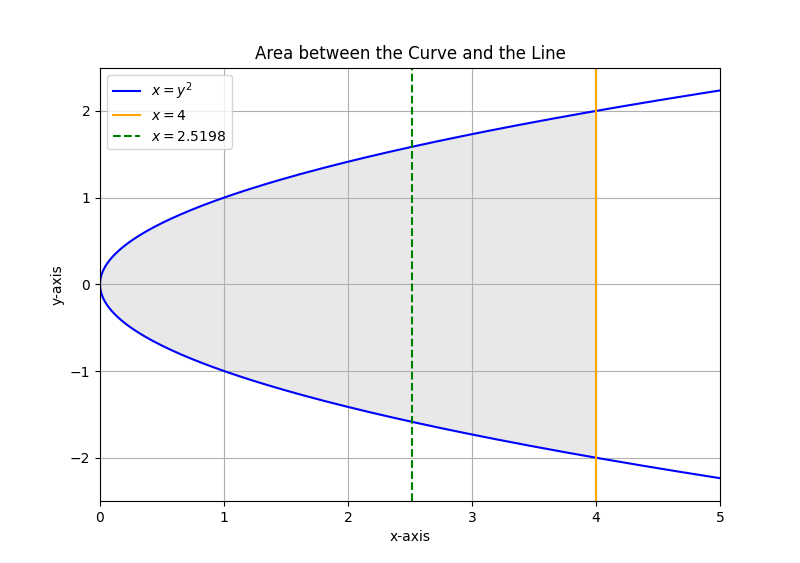
\includegraphics[width=0.7\linewidth]{fig/Figure_1.png}
		\caption{}
        \label{stemplot}
\end{figure}

    
 \end{document}
